\documentclass[../../compsys.tex]{subfiles}
\begin{document}
\raggedbottom
\chapter{L12 – Network System Calls \& the Internet}
\vfill
\section{From End–Systems to Processes}
Every computer attached to the Internet that exchanges messages is called an \textbf{end-system}.  
\begin{itemize}
  \item[-] \textbf{Client process}: issues \emph{requests}.  
  \item[-] \textbf{Server process}: generates \emph{responses}.  
\end{itemize}
Thus, the words \emph{client} and \emph{server} are used both for the \emph{processes} and for the \emph{machines} executing them.

\subsection{Naming a Process}
A process is uniquely identified by the pair  
\[
  \texttt{IP address} : \texttt{port number}
\]
\begin{description}
  \item[IP address] (e.g.\ \texttt{8.8.8.8}) – identifies the end-system.  
  \item[Port number] (e.g.\ \texttt{53}) – identifies the process on that end-system.  Certain services have \emph{well-known ports} (DNS uses port 53).
\end{description}
\subsubsection{Some definitions}\small
\begin{description}
  \item[End-system] A host connected to the Internet that can send/receive packets.  
  \item[Socket] A file descriptor returned by \texttt{socket()}; used with \texttt{sendto()} and \texttt{recvfrom()} instead of \texttt{read()} and \texttt{write()}.  
  \item[Well-known port] A globally agreed port number reserved for a specific application‐level protocol (e.g.\ port 53 for DNS).  
\end{description}
\newpage
\subsection{Network System Calls}
The following POSIX calls allow a user process to exchange messages with a remote peer:
\subsubsection{Server‐side calls}
\begin{enumerate}
  \item \texttt{socket()} – create a network endpoint and obtain a \textbf{socket}, a special file descriptor.
  \item \texttt{bind()} – register the local process name \texttt{[IP,\,port]} with the kernel (e.g.\ \texttt{[8.8.8.8,53]}).
  \item \texttt{recvfrom()} – retrieve an arriving request; the kernel fills in the client's \texttt{[IP,\,port]}.
  \item \texttt{sendto()} – transmit a response back to the requesting client.
  \item \texttt{close()} – release the socket when no more requests should be served.
\end{enumerate}

\subsubsection{Client‐side calls}
\begin{enumerate}
  \item \texttt{socket()} – create a socket (no fixed port required).
  \item \texttt{sendto()} – hand the kernel the request packet and the server's address (e.g.\ \texttt{[8.8.8.8,53]}).
  \item \texttt{recvfrom()} – wait for (or poll for) the matching response.
  \item \texttt{close()} – terminate communication once all responses are received.
\end{enumerate}

\paragraph{Blocking vs.\ Non-blocking}  Each call (most notably \texttt{recvfrom()}) may be invoked in \textbf{blocking} mode (the kernel puts the process to sleep until data arrives) or \textbf{non-blocking} mode (the call returns immediately with an error code such as \texttt{EAGAIN} if no data is ready).\\[15px]
\subsection{Example Network Flow}
\begin{minipage}[t]{0.45\textwidth}
    \small
\subsubsection*{Client $\rightarrow$ Server (Request)}
\vspace{10px}
\begin{center}
  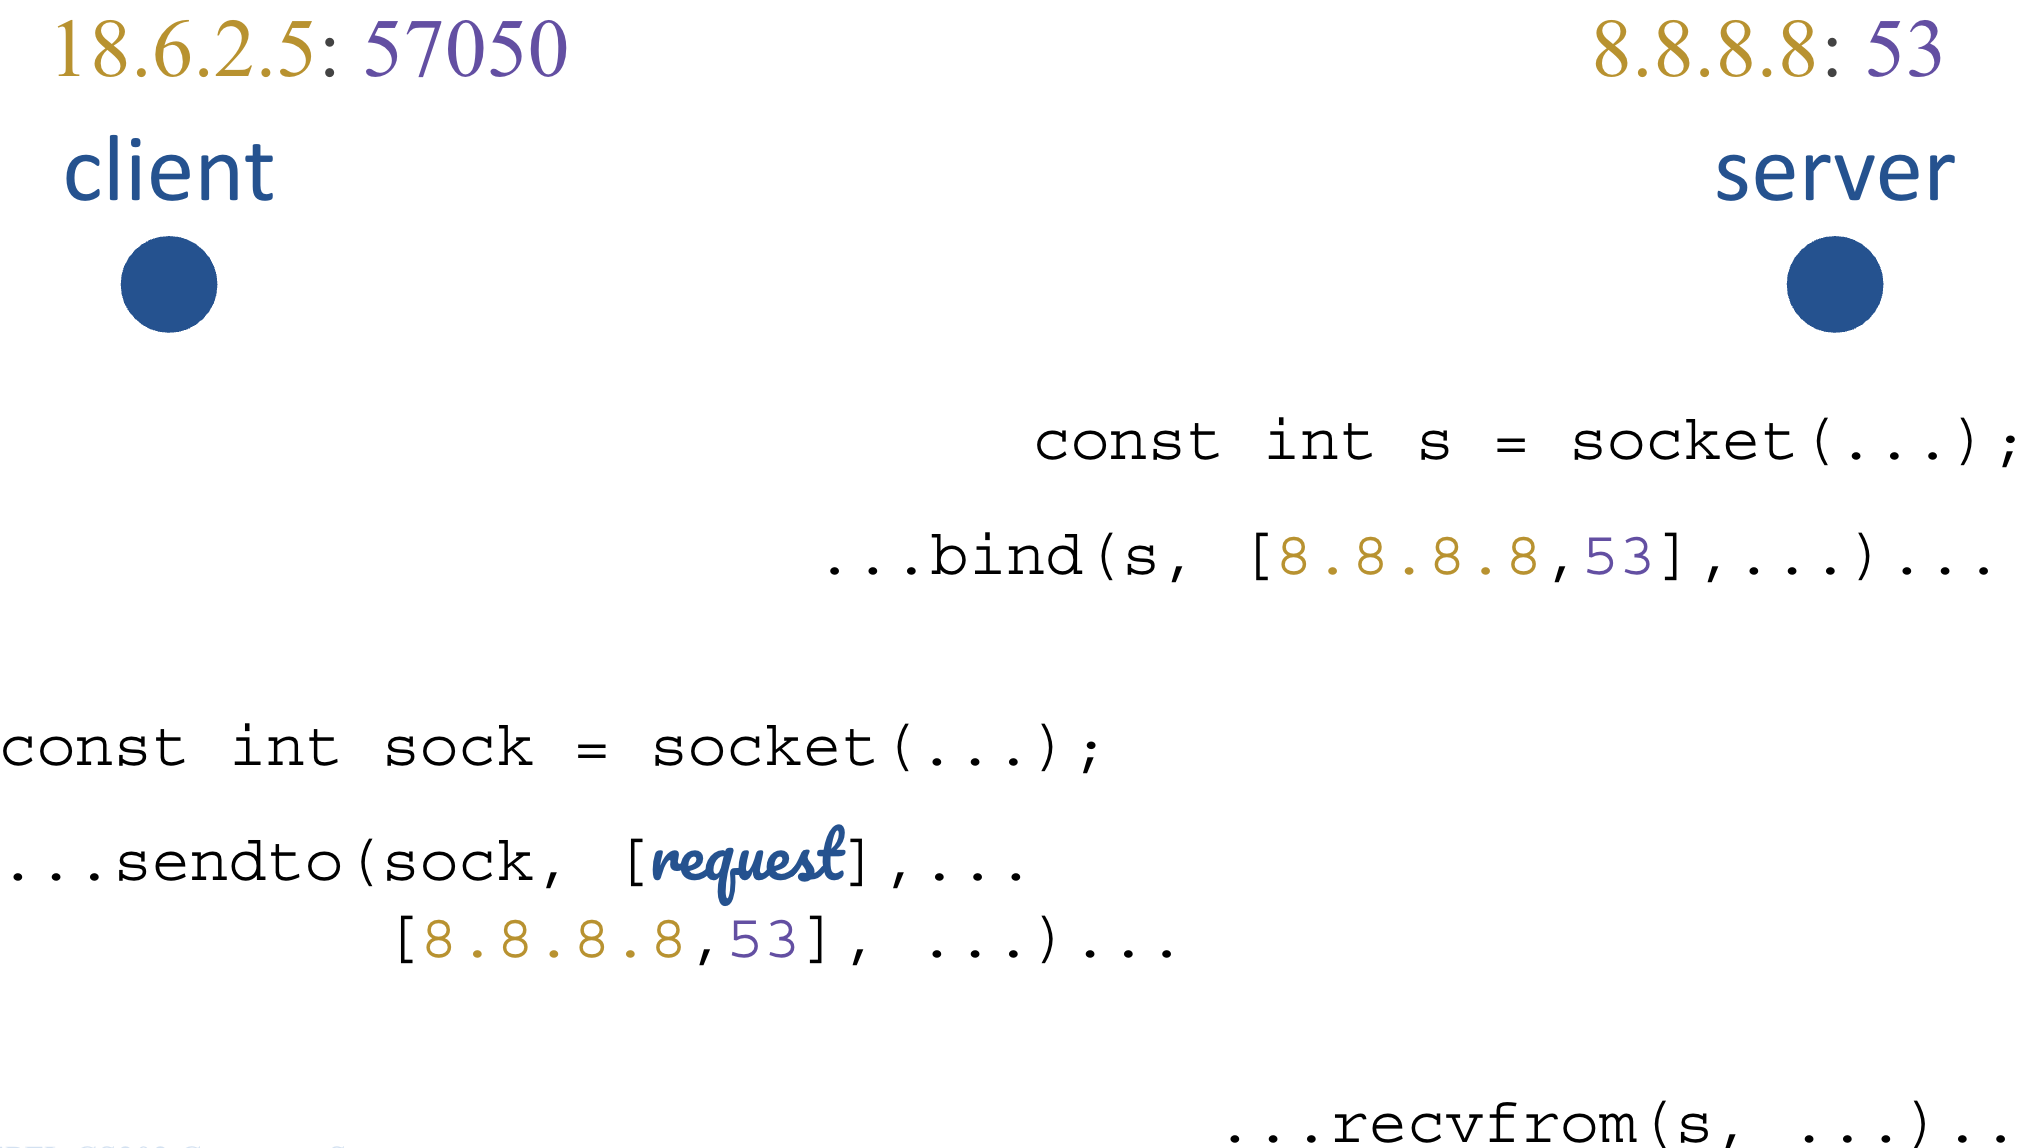
\includegraphics[width=0.7\textwidth]{images/client-to-server-syscalls.png}
\end{center}

\begin{enumerate}
  \item Client issues \texttt{socket()} then \texttt{sendto()}(\textit{request},\,[8.8.8.8,53]).
  \item Kernel consults its routing tables and places the UDP datagram on the wire.
  \item Server's NIC receives the packet; the kernel matches \texttt{[8.8.8.8,53]} to the waiting socket produced by \texttt{bind()}.
  \item Server process unblocks from \texttt{recvfrom()} and obtains both the request data and the client's return address.
\end{enumerate}
\end{minipage}
\begin{minipage}[t]{0.45\textwidth}
    \small
\subsubsection*{Server $\rightarrow$ Client (Response)}
\vspace{10px}
\begin{center}
  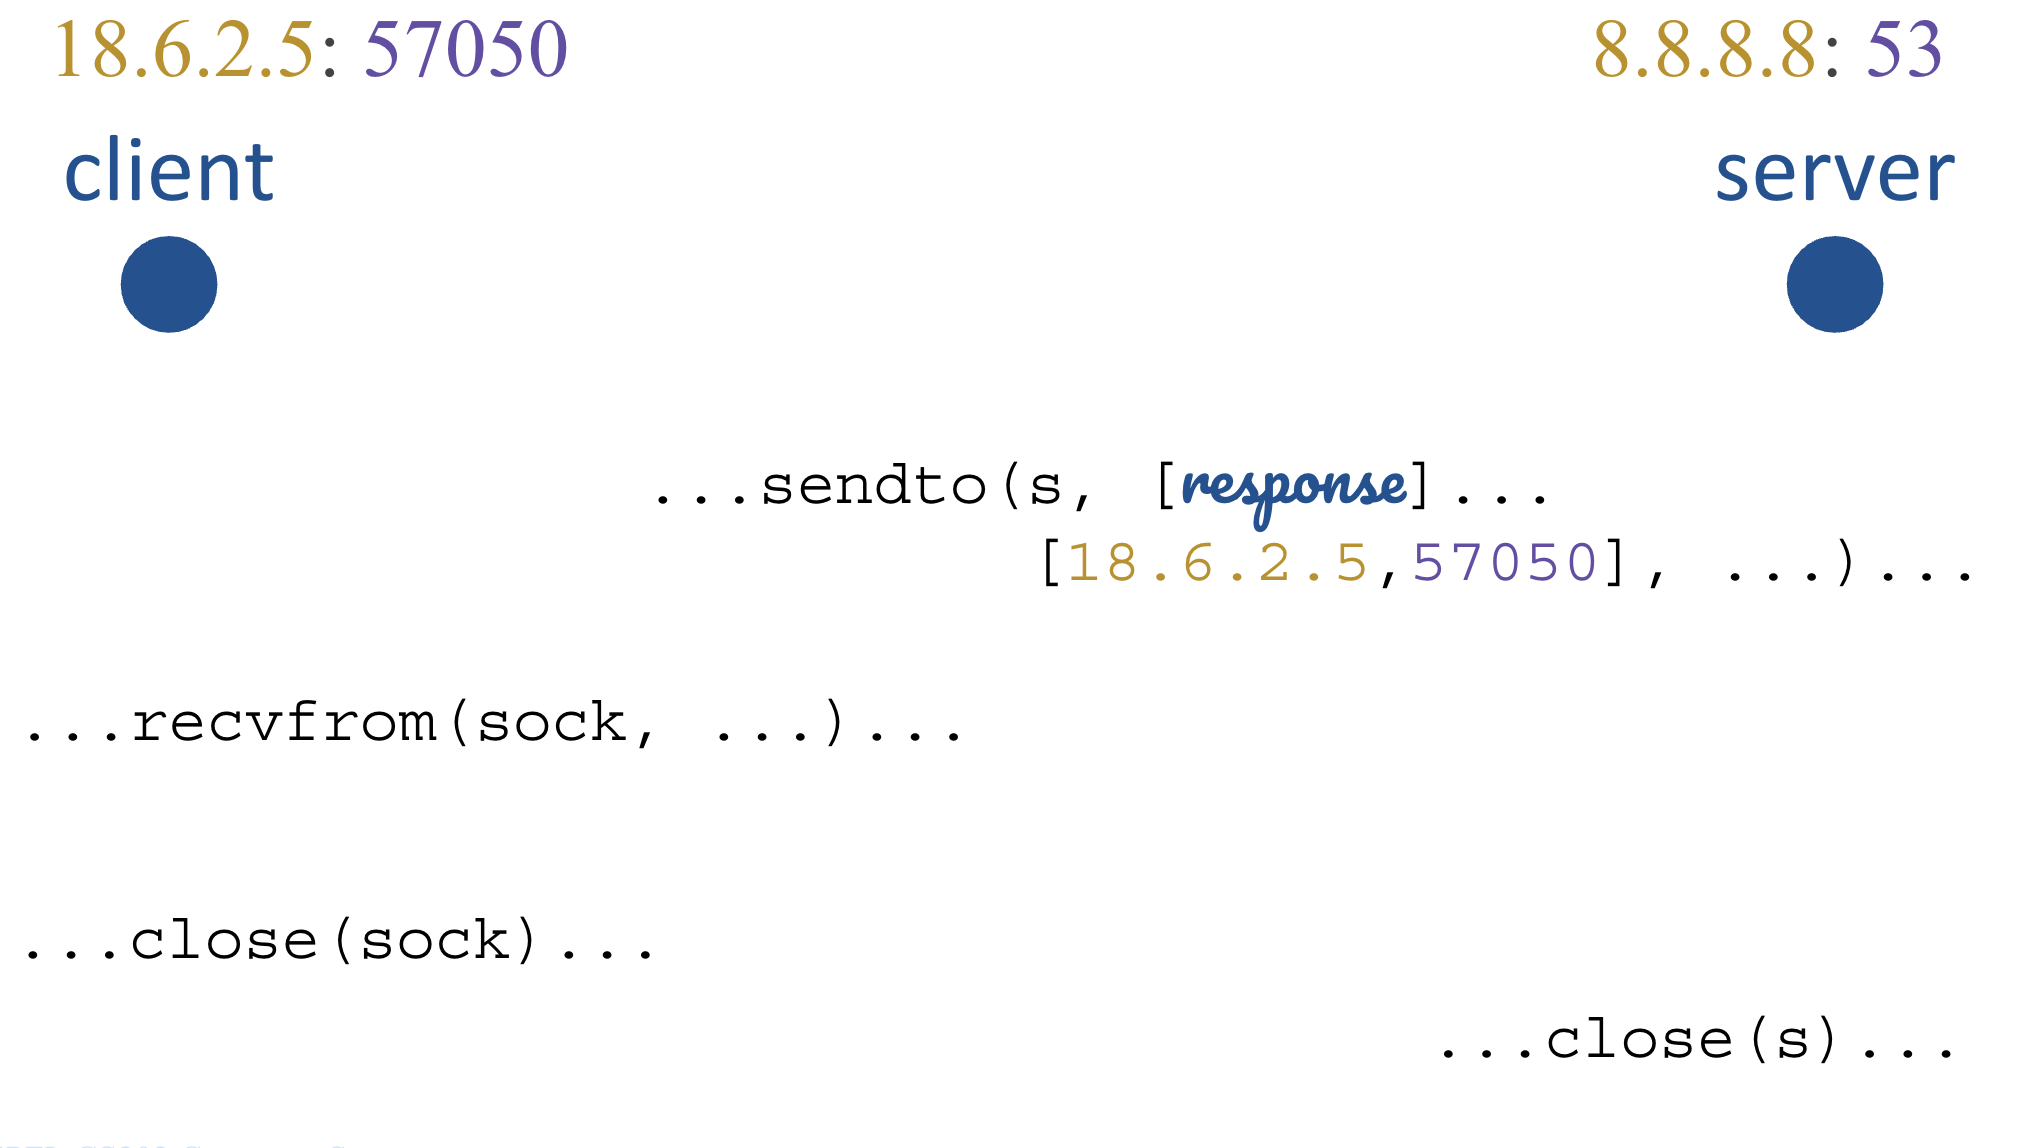
\includegraphics[width=0.7\textwidth]{images/server-to-client-syscalls.png}
\end{center}

\begin{enumerate}
  \item Server calls \texttt{sendto()}(\textit{response},\,[18.6.2.5,57050]).
  \item Packet traverses the network back to the client.
  \item Client's kernel delivers the datagram to the waiting socket; \texttt{recvfrom()} returns the response.
  \item Client invokes \texttt{close()}.  (Whether any data is sent upon \texttt{close()} depends on the socket type—topic for a later lecture.)
  \item Server eventually calls \texttt{close()} when it no longer wishes to serve further requests.
\end{enumerate}
\end{minipage}
%--------------------------------------------------------------------
\section{Internet Components}\label{sec:intcomp}
This section introduces the most common ways an \textbf{end-system}
(e.g.\ your laptop) reaches the global Internet.  
For every access technology we list the physical path, the achievable data
rate, and the main engineering trade-offs.

%--------------------------------------------------------------------
\subsection{Access via the Public Switched Telephone Network}
A typical home setup places the laptop behind a
\emph{DSL/Fiber modem–router} that terminates the household
telephone line and relays traffic to the \emph{central office}
a few kilometres away.

\begin{center}
  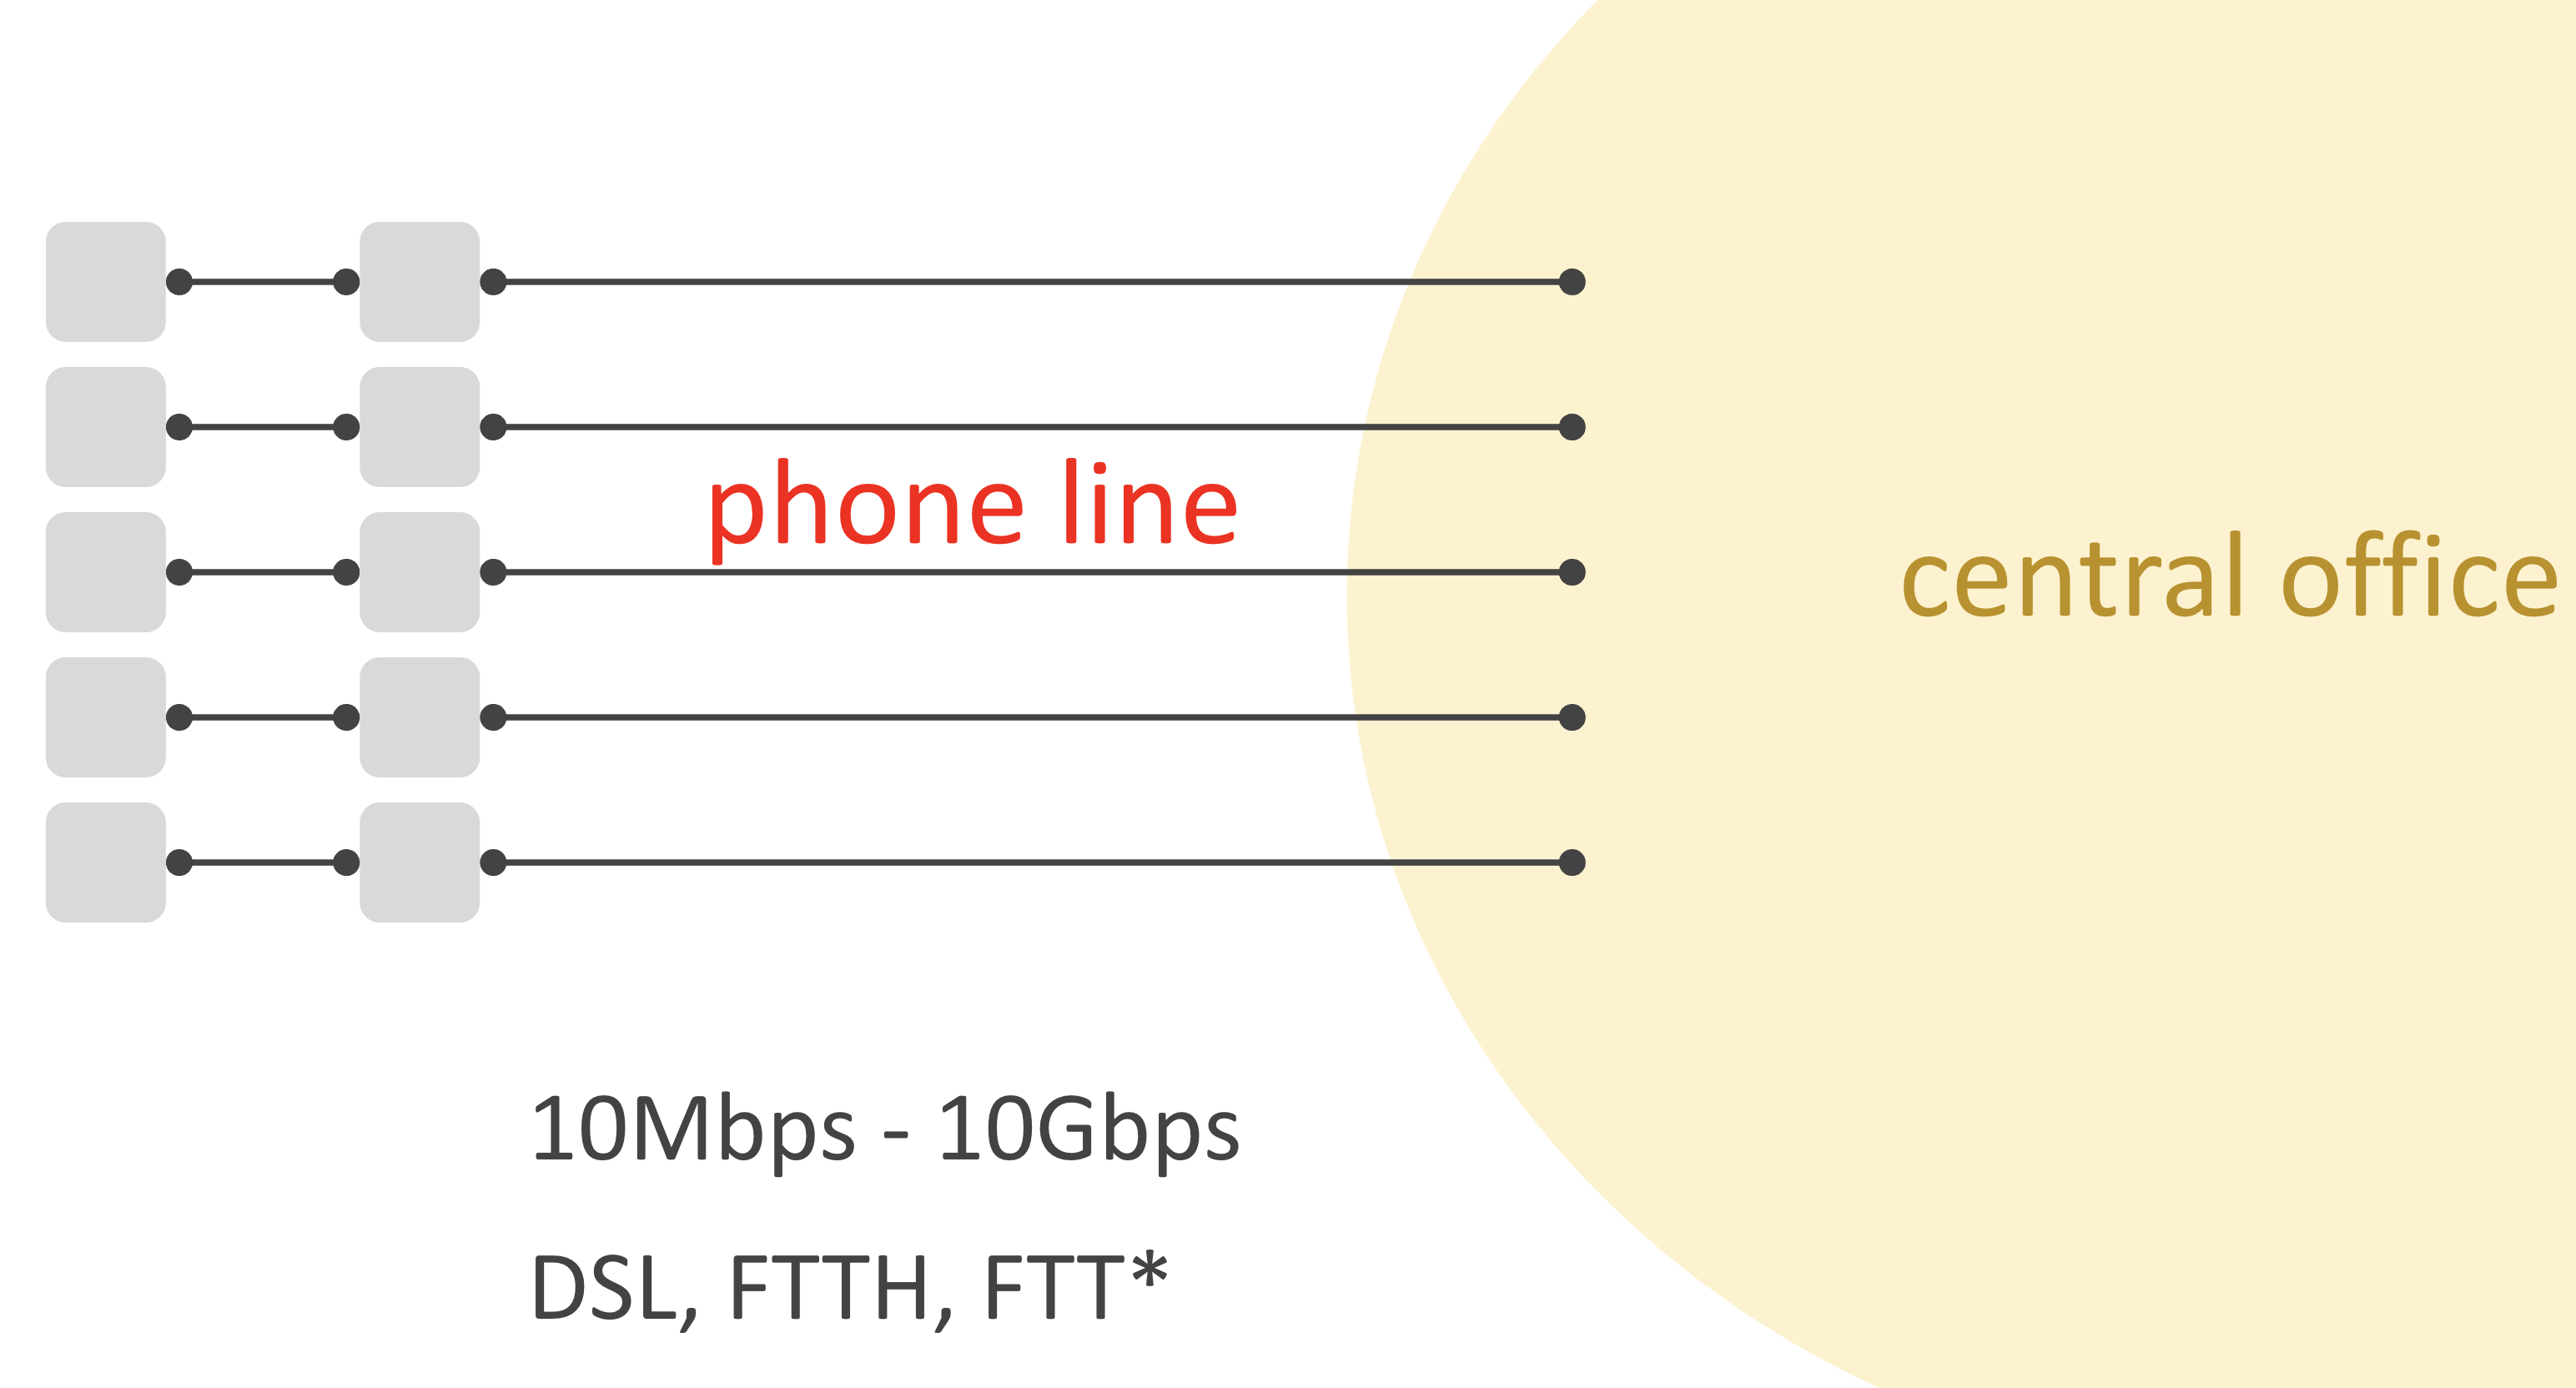
\includegraphics[width=0.6\textwidth]{images/phone-line.png}
\end{center}

\begin{enumerate}
  \item \textbf{Path}: Laptop $\rightarrow$ Modem/Router $\rightarrow$
        Copper / Fiber local loop $\rightarrow$ Central Office $\rightarrow$ Internet.
  \item \textbf{Rate}: 10--10,000 Mbps 
        (material and DSL/Fiber technology dependent).
  \item \textbf{Why legacy copper?}
        \begin{itemize}
          \item Incumbent telcos \emph{already own} a wire to every
                household\,—\,a compelling business advantage.
          \item Pulling new fibre is capital-intensive; upgrades therefore
                proceed gradually (\emph{FTTH}, \emph{FTTB}, \emph{FTTC}, \dots).
        \end{itemize}
\end{enumerate}

\begin{description}
  \item[End-system] Any device exchanging packets over the Internet.
  \item[Modem] A specialised \emph{packet switch} that adapts IP packets
               to the physical characteristics of the telephone line.
\end{description}


%--------------------------------------------------------------------
\subsection{Access via the Cable TV Network}
A second option reuses the coaxial cable that once delivered only
television signals.

\begin{center}
  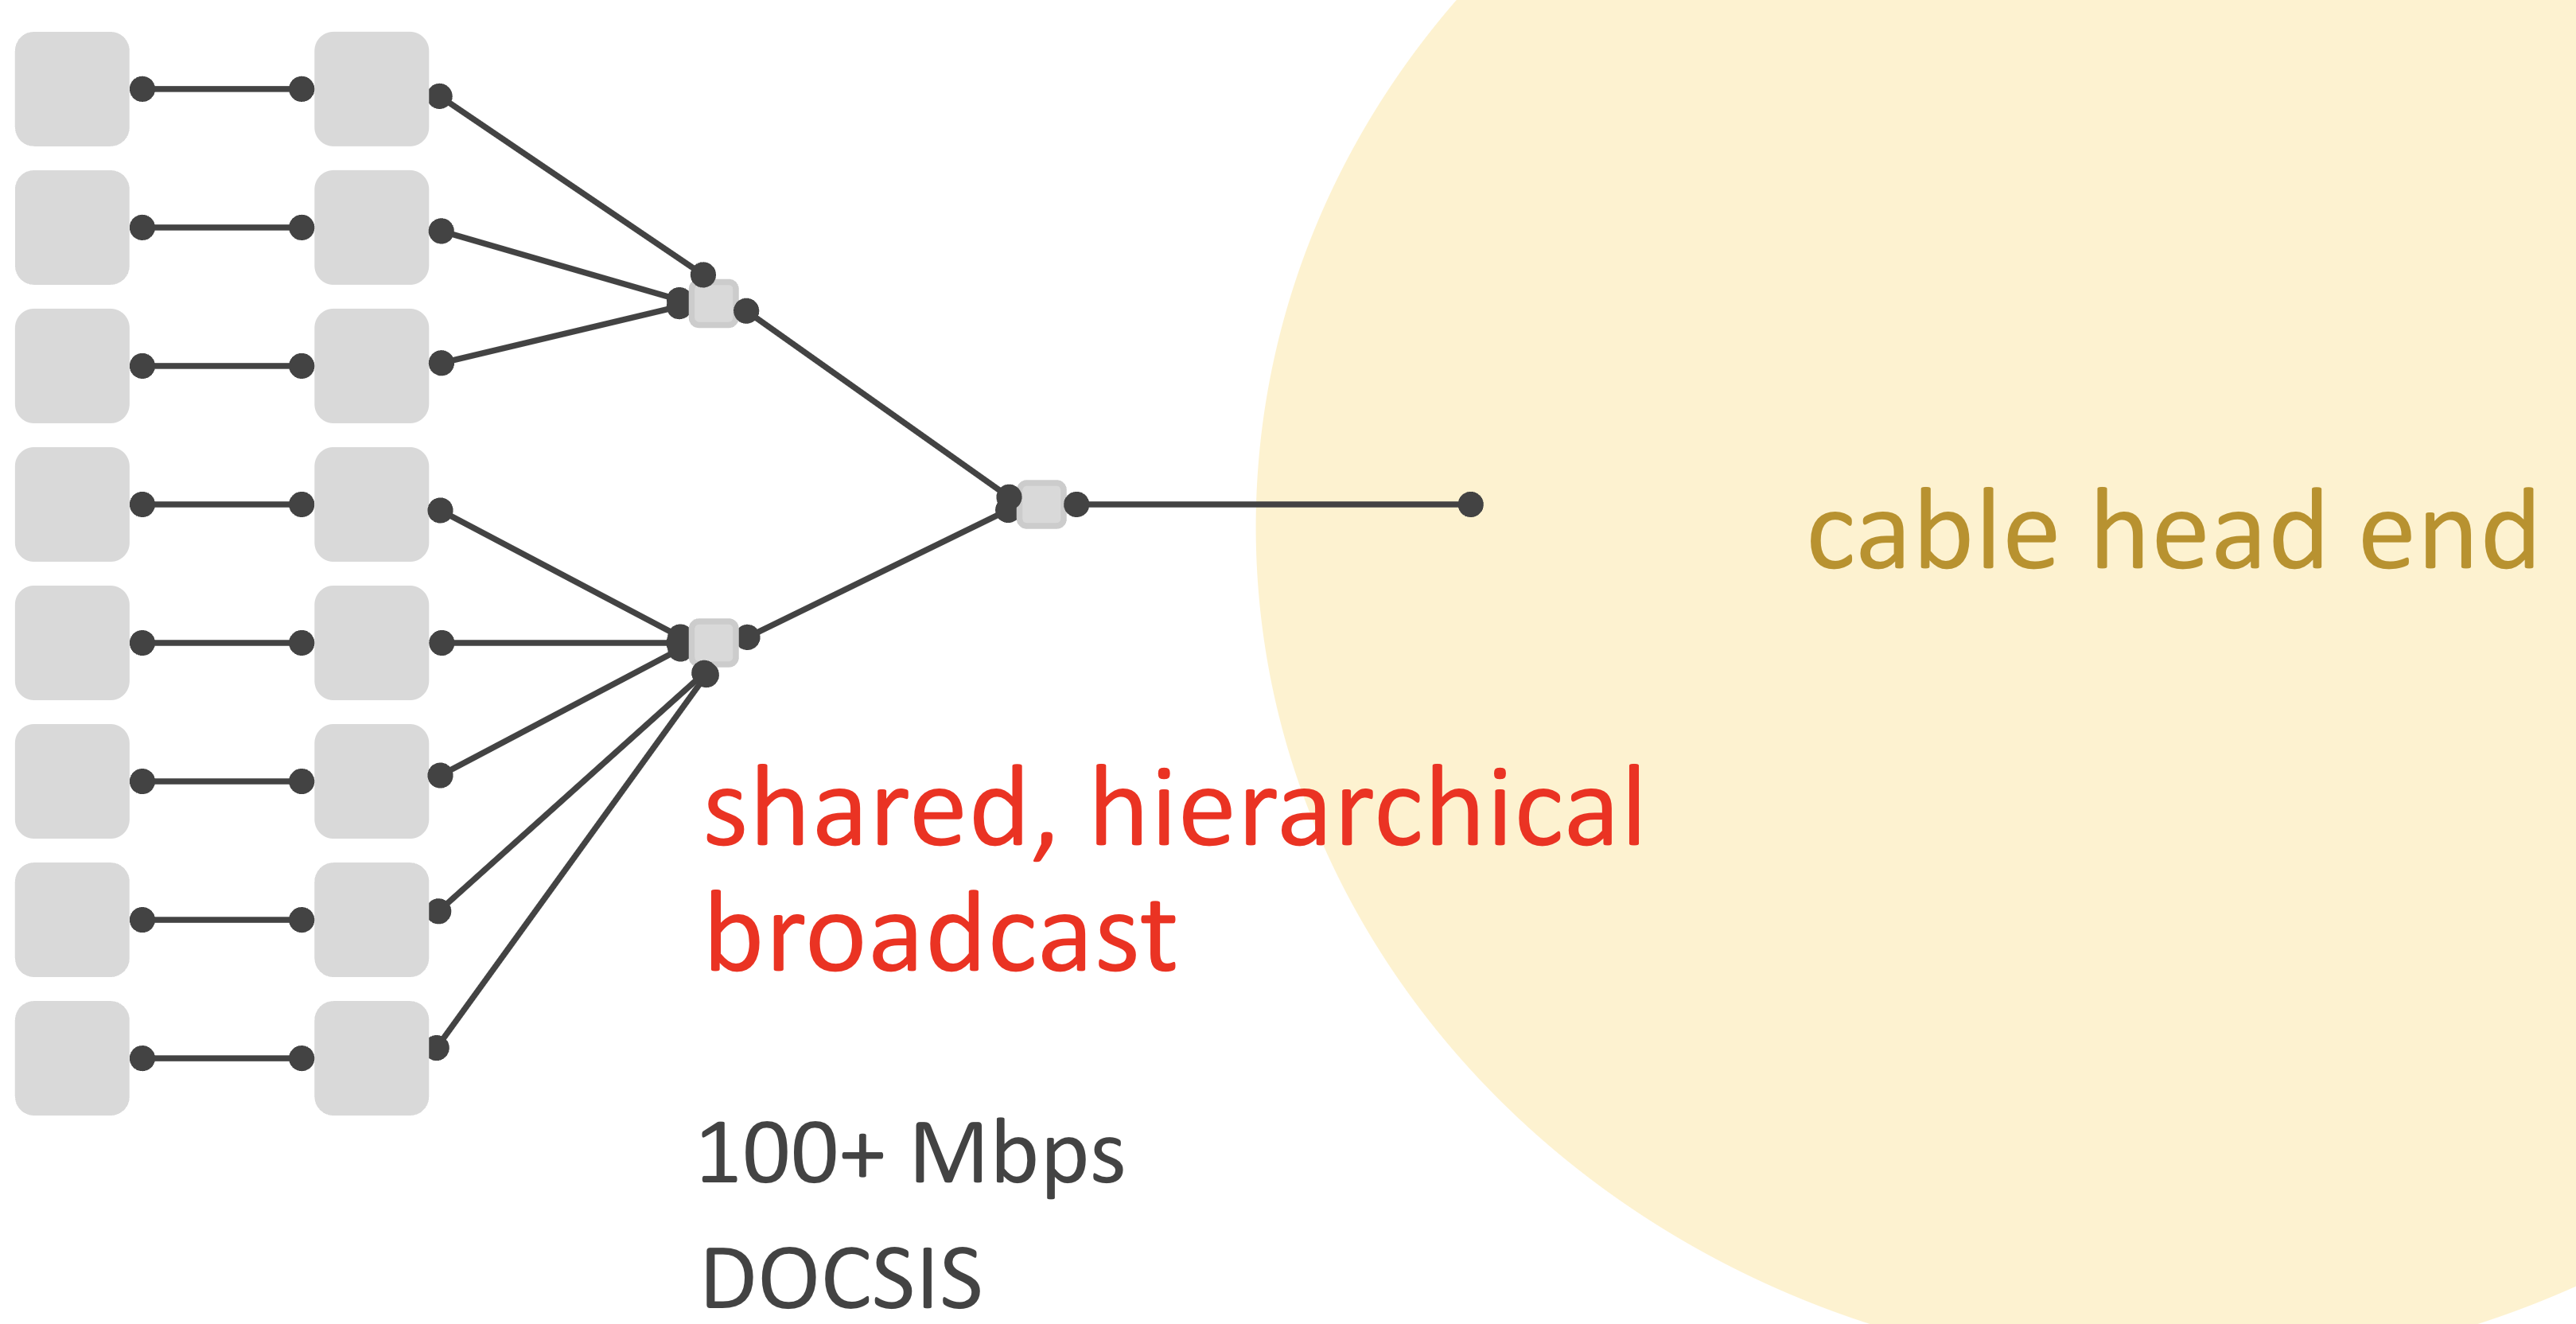
\includegraphics[width=0.6\textwidth]{images/tv-line.png}
\end{center}

\begin{enumerate}
  \item \textbf{Path}: Laptop $\rightarrow$ Cable Modem/Router $\rightarrow$
        Coaxial tree $\rightarrow$ \emph{Cable Head-End} $\rightarrow$ Internet.
  \item \textbf{Rate}: Typically 100--1,000 Mbps.
  \item \textbf{Key differences to DSL}:
        \begin{enumerate}
          \item \textit{Shared medium} — the last-mile coax is shared by
                all subscribers on the tree; throughput per user can drop
                at peak times (e.g.\ Saturday night).
          \item \textit{Broadcast medium} — frames sent by the head-end are
                physically delivered to \emph{every} household on the tree.
        \end{enumerate}
\end{enumerate}

\begin{description}
  \item[Shared medium] Multiple end-systems contend for the same link.
  \item[Broadcast medium] A single transmission is received by all nodes
        on the medium.
\end{description}


%--------------------------------------------------------------------
\subsection{Access via a Point of Presence (PoP)}
Enterprise campuses and data-centres aggregate thousands of machines
through a switched hierarchy that ultimately connects to an
\textbf{ISP Point of Presence (PoP)}.
\begin{center}
  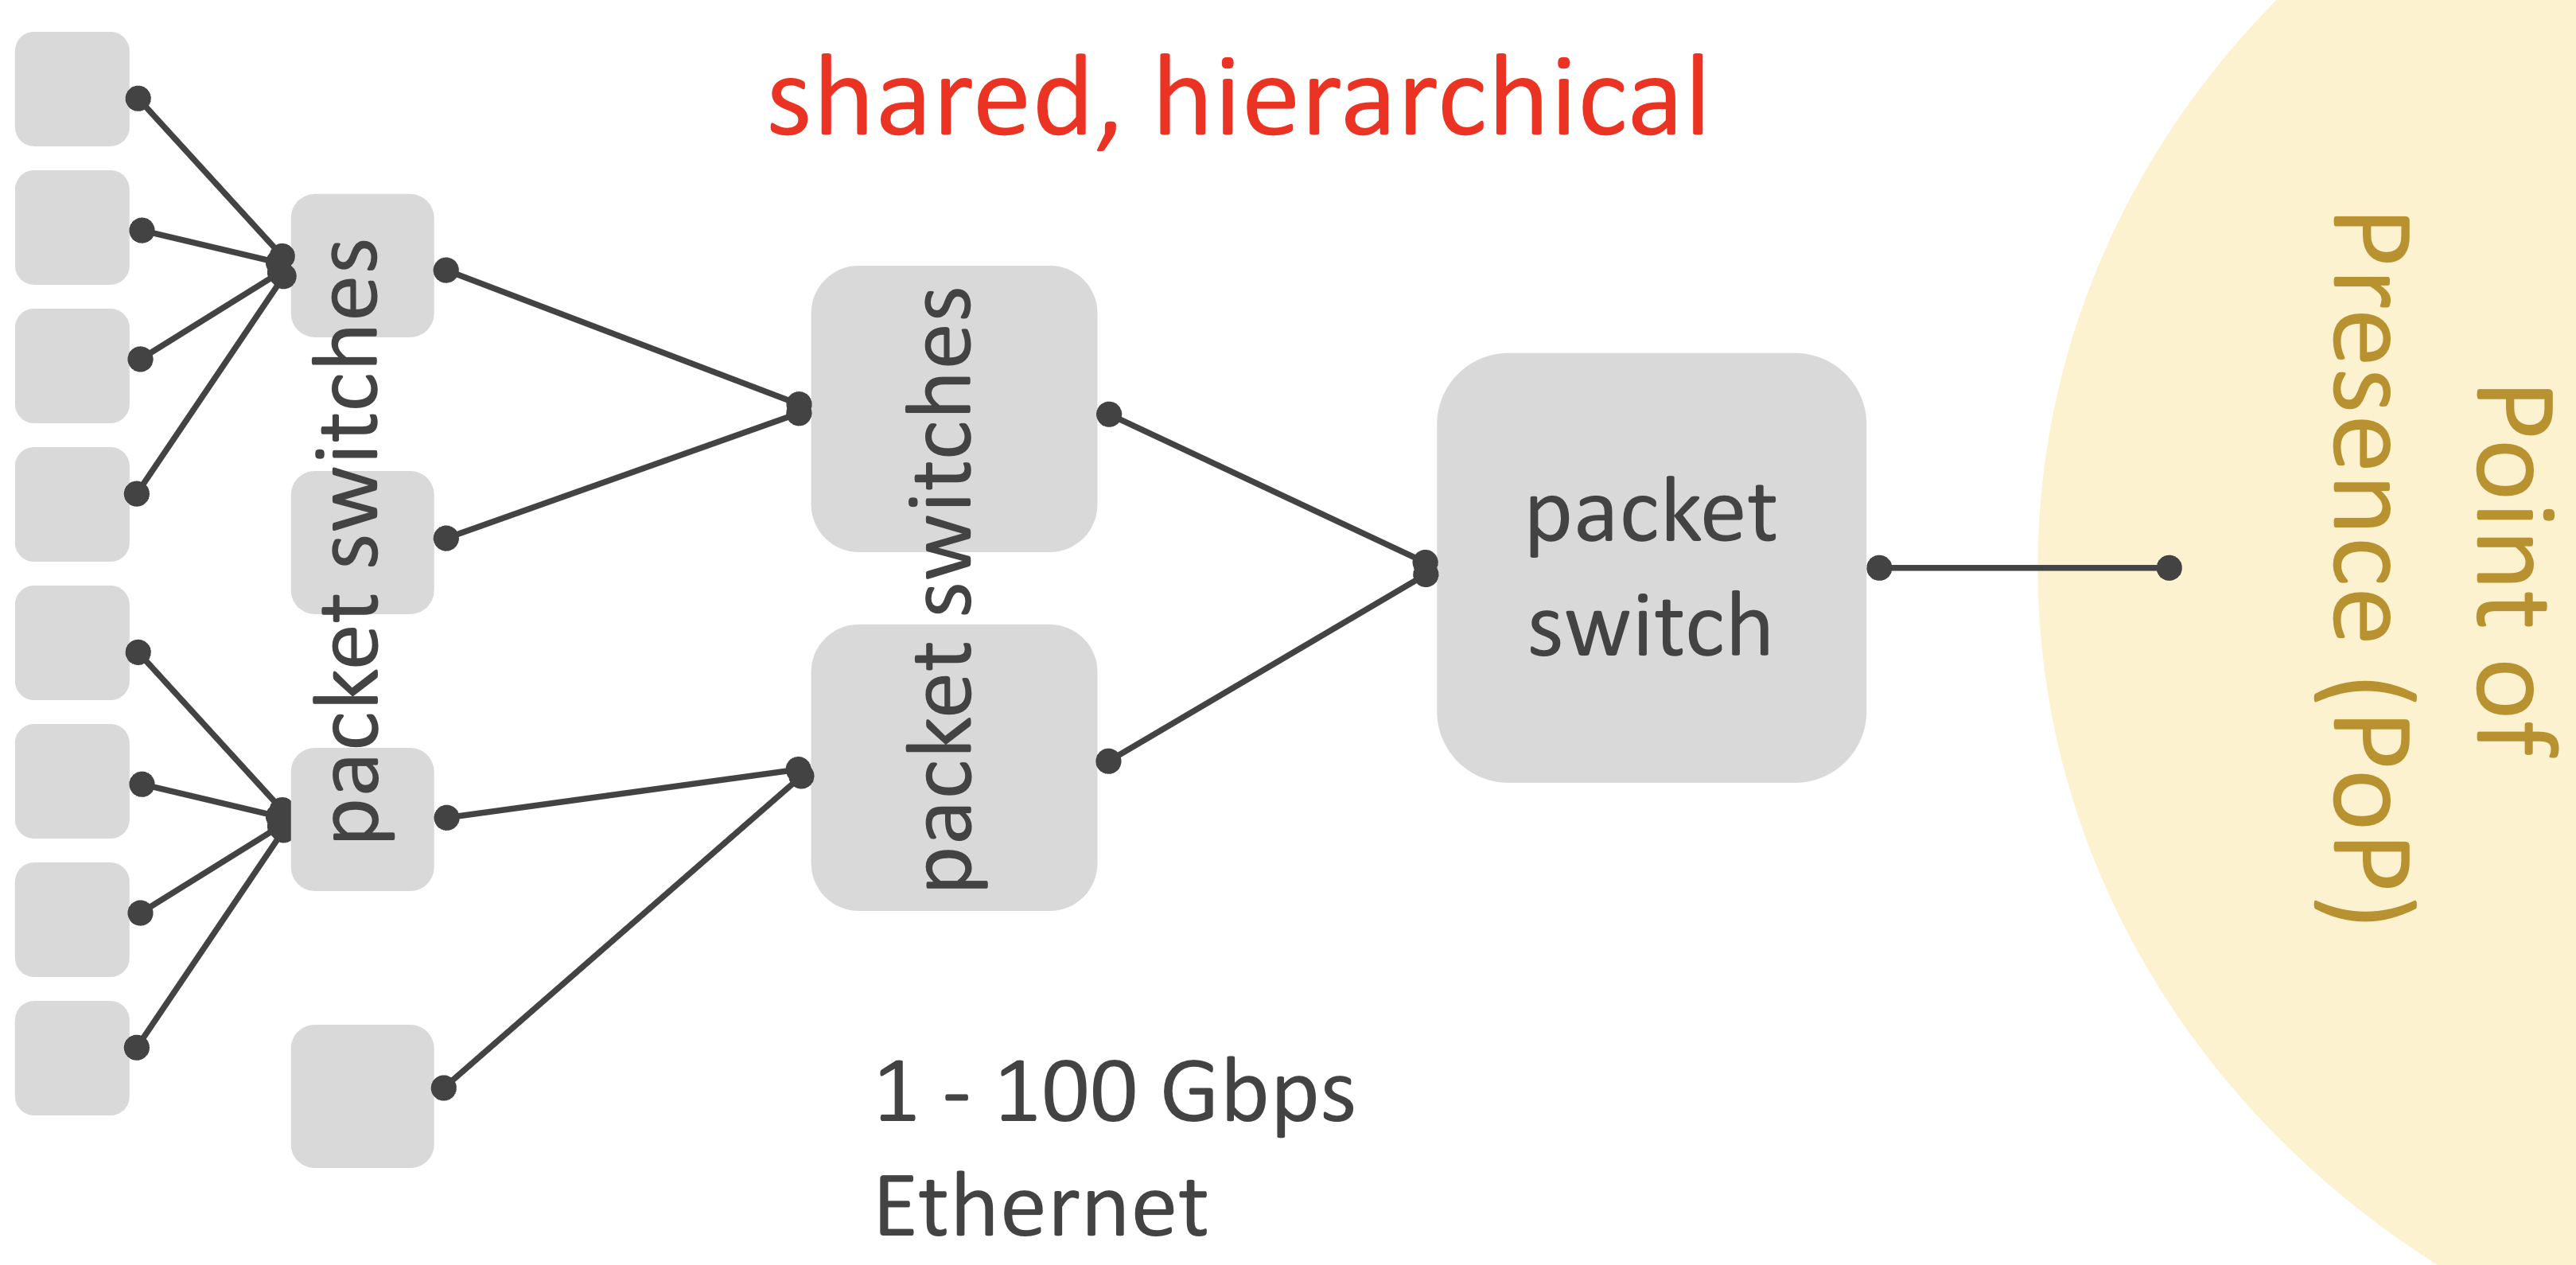
\includegraphics[width=0.6\textwidth]{images/pop.png}
\end{center}

\begin{enumerate}
  \item \textbf{Path}: Workstation $\rightarrow$ Access switch
        $\rightarrow$ Aggregation/Core switch $\rightarrow$ PoP
        $\rightarrow$ Internet.
  \item \textbf{Rate}: 1--100 Gbps per link inside the site.
  \item \textbf{Hierarchy}: Many small switches feed fewer, higher-capacity
        switches, reducing cost while maintaining performance.
\end{enumerate}

\begin{description}
  \item[PoP] The interface between a customer network (campus,
        enterprise, data-centre) and an Internet Service Provider.
\end{description}


%--------------------------------------------------------------------
\subsubsection{Summary}\label{sssec:summary}
\begin{itemize}
  \item[-] \textbf{Access technologies}: DSL/Fiber over phone lines,
        Cable-TV coax, cellular, satellite, campus PoP, \dots
  \item[-] \textbf{Ownership}: Each path segment is operated by an
        \emph{Internet Service Provider (ISP)} such as a telco
        (Swisscom), a cable operator (UPC/Sunrise), or a research
        network (SWITCH).
  \item[-] \textbf{Design heuristic}: When extending connectivity,
        always ask:
        \begin{enumerate}
          \item What infrastructure already exists?
          \item Which media are users accustomed to paying for?
        \end{enumerate}
        Leveraging existing assets often yields the most economical
        solution.
\end{itemize}
\newpage
%---------------------------------------------------------------
\section{Internet Service Providers (ISPs)}\label{sec:isps}
Every end-system ultimately reaches the global Internet through one or
more \textbf{Internet Service Providers (ISPs)}.  
To scale worldwide connectivity, ISPs organise themselves in a \emph{three-tier
hierarchy} linked by specific business agreements.

%---------------------------------------------------------------
\subsection{Why a Hierarchy?}\label{subsec:whyhier}
Directly wiring every pair of the world's access networks is infeasible
(thousands of telcos, cable operators, universities, enterprises,~\dots).
Instead, ISPs form a multi-level structure:
\begin{center}
    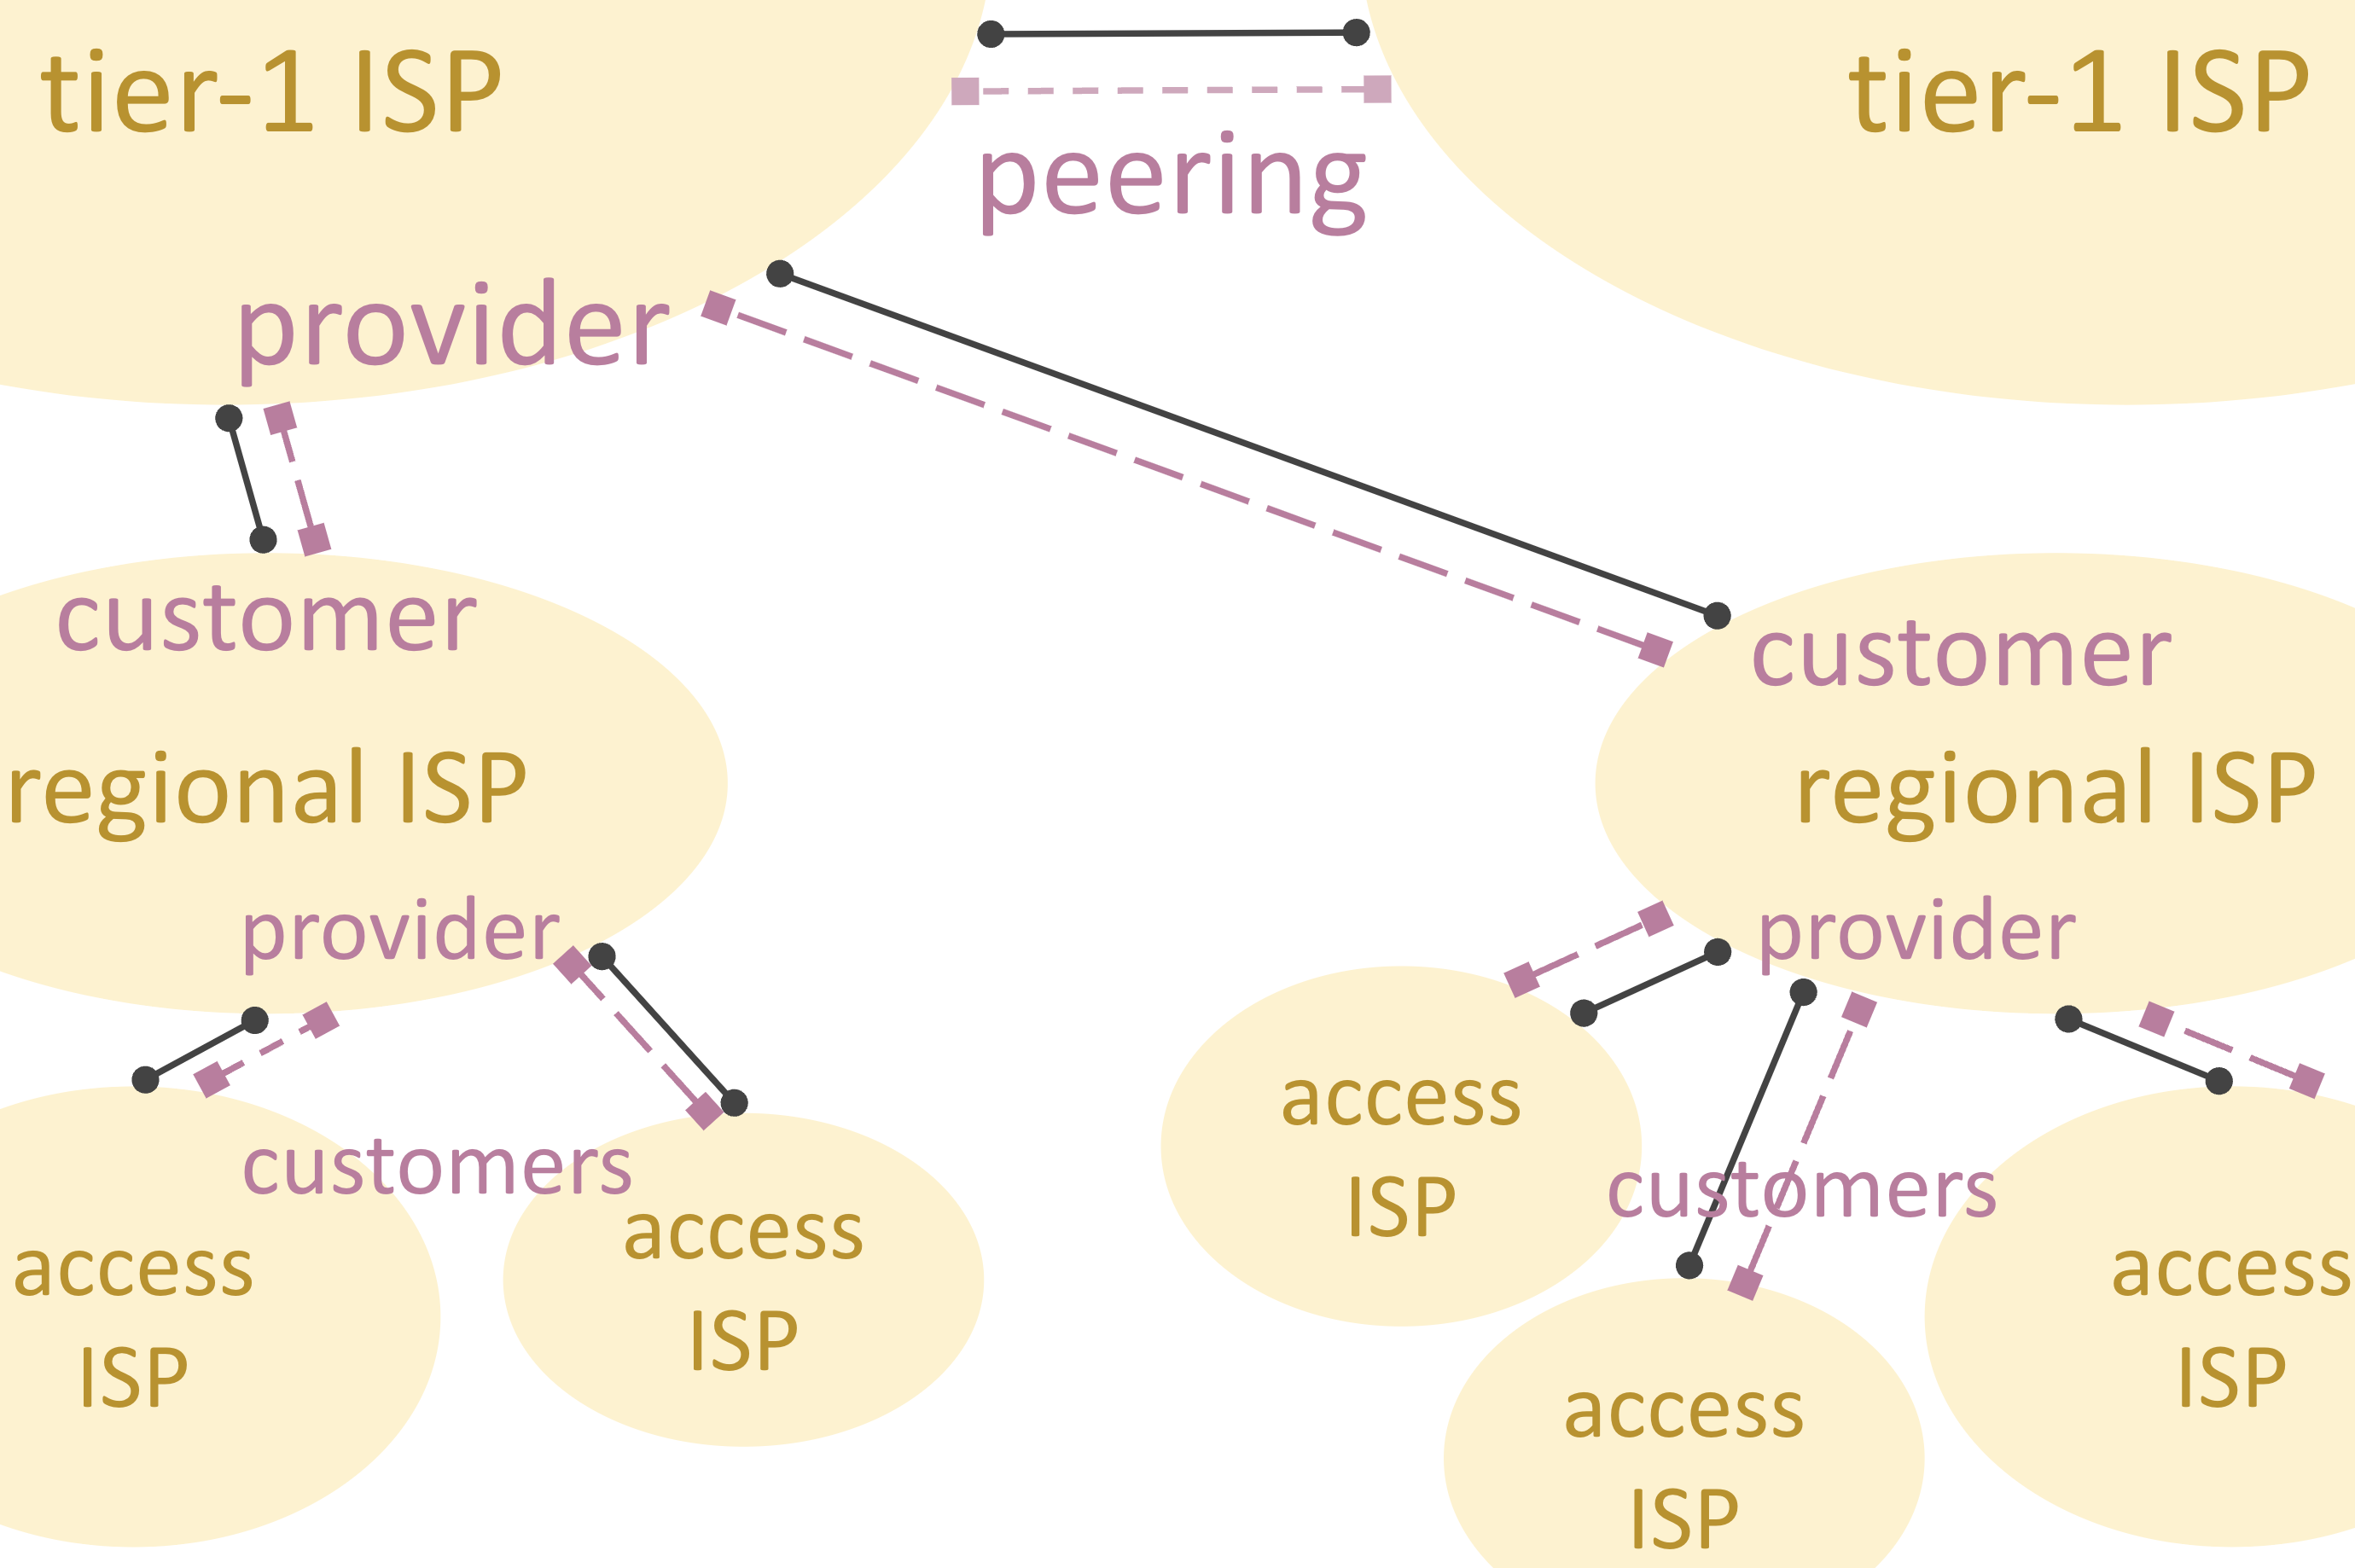
\includegraphics[width=0.60\textwidth]{images/isp-hiearchy.png}
  \end{center}
  
\begin{enumerate}
  \item \textbf{Access ISPs} ― interface with end-systems (e.g.\ Swisscom,
        Sunrise).
  \item \textbf{Regional ISPs} ― aggregate many access ISPs within a
        country or region.
  \item \textbf{Tier-1 ISPs} ― few, globe-spanning backbones that can
        reach every network without paying another provider.
\end{enumerate}

\begin{definition}
  \textbf{Customer–provider relationship}: the lower-tier ISP
  (\emph{customer}) pays the higher-tier ISP (\emph{provider}) for global
  reachability.
\end{definition}

%---------------------------------------------------------------
\subsection{Peering Agreements}\label{subsec:peering}
When two ISPs exchange large, roughly balanced traffic volumes, they may
bypass providers and interconnect as \textbf{peers}:

\begin{itemize}
  \item[-] \emph{Settlement-free peering}: each party carries the other's
        traffic at no cost.
  \item[-] \emph{Paid peering}: one ISP compensates the other if traffic
        is highly asymmetric.
\end{itemize}

Peering can occur at \emph{any} tier (access $\leftrightarrow$ access, regional $\leftrightarrow$
regional, tier-1  $\leftrightarrow$ tier-1) whenever it is economically attractive.

%---------------------------------------------------------------
\subsection{Internet eXchange Points (IXPs)}\label{subsec:ixp}
ISPs rarely drag a private cable to every partner.  
Instead, they each attach \emph{one} high-speed link to a neutral
facility called an \textbf{IXP}―essentially a massive Ethernet switch
where multiple ISPs exchange traffic.

\begin{description}
  \item[IXP] Neutral switching fabric that enables many bilateral or
        multilateral interconnections through a single physical port.
\end{description}

%---------------------------------------------------------------
\subsection{Content/Cloud Providers as Networks}\label{subsec:ccp}
Companies such as Google, Microsoft, Amazon, and Meta evolved from
regular customers of ISPs into operators of near-global backbones:

\begin{center}
    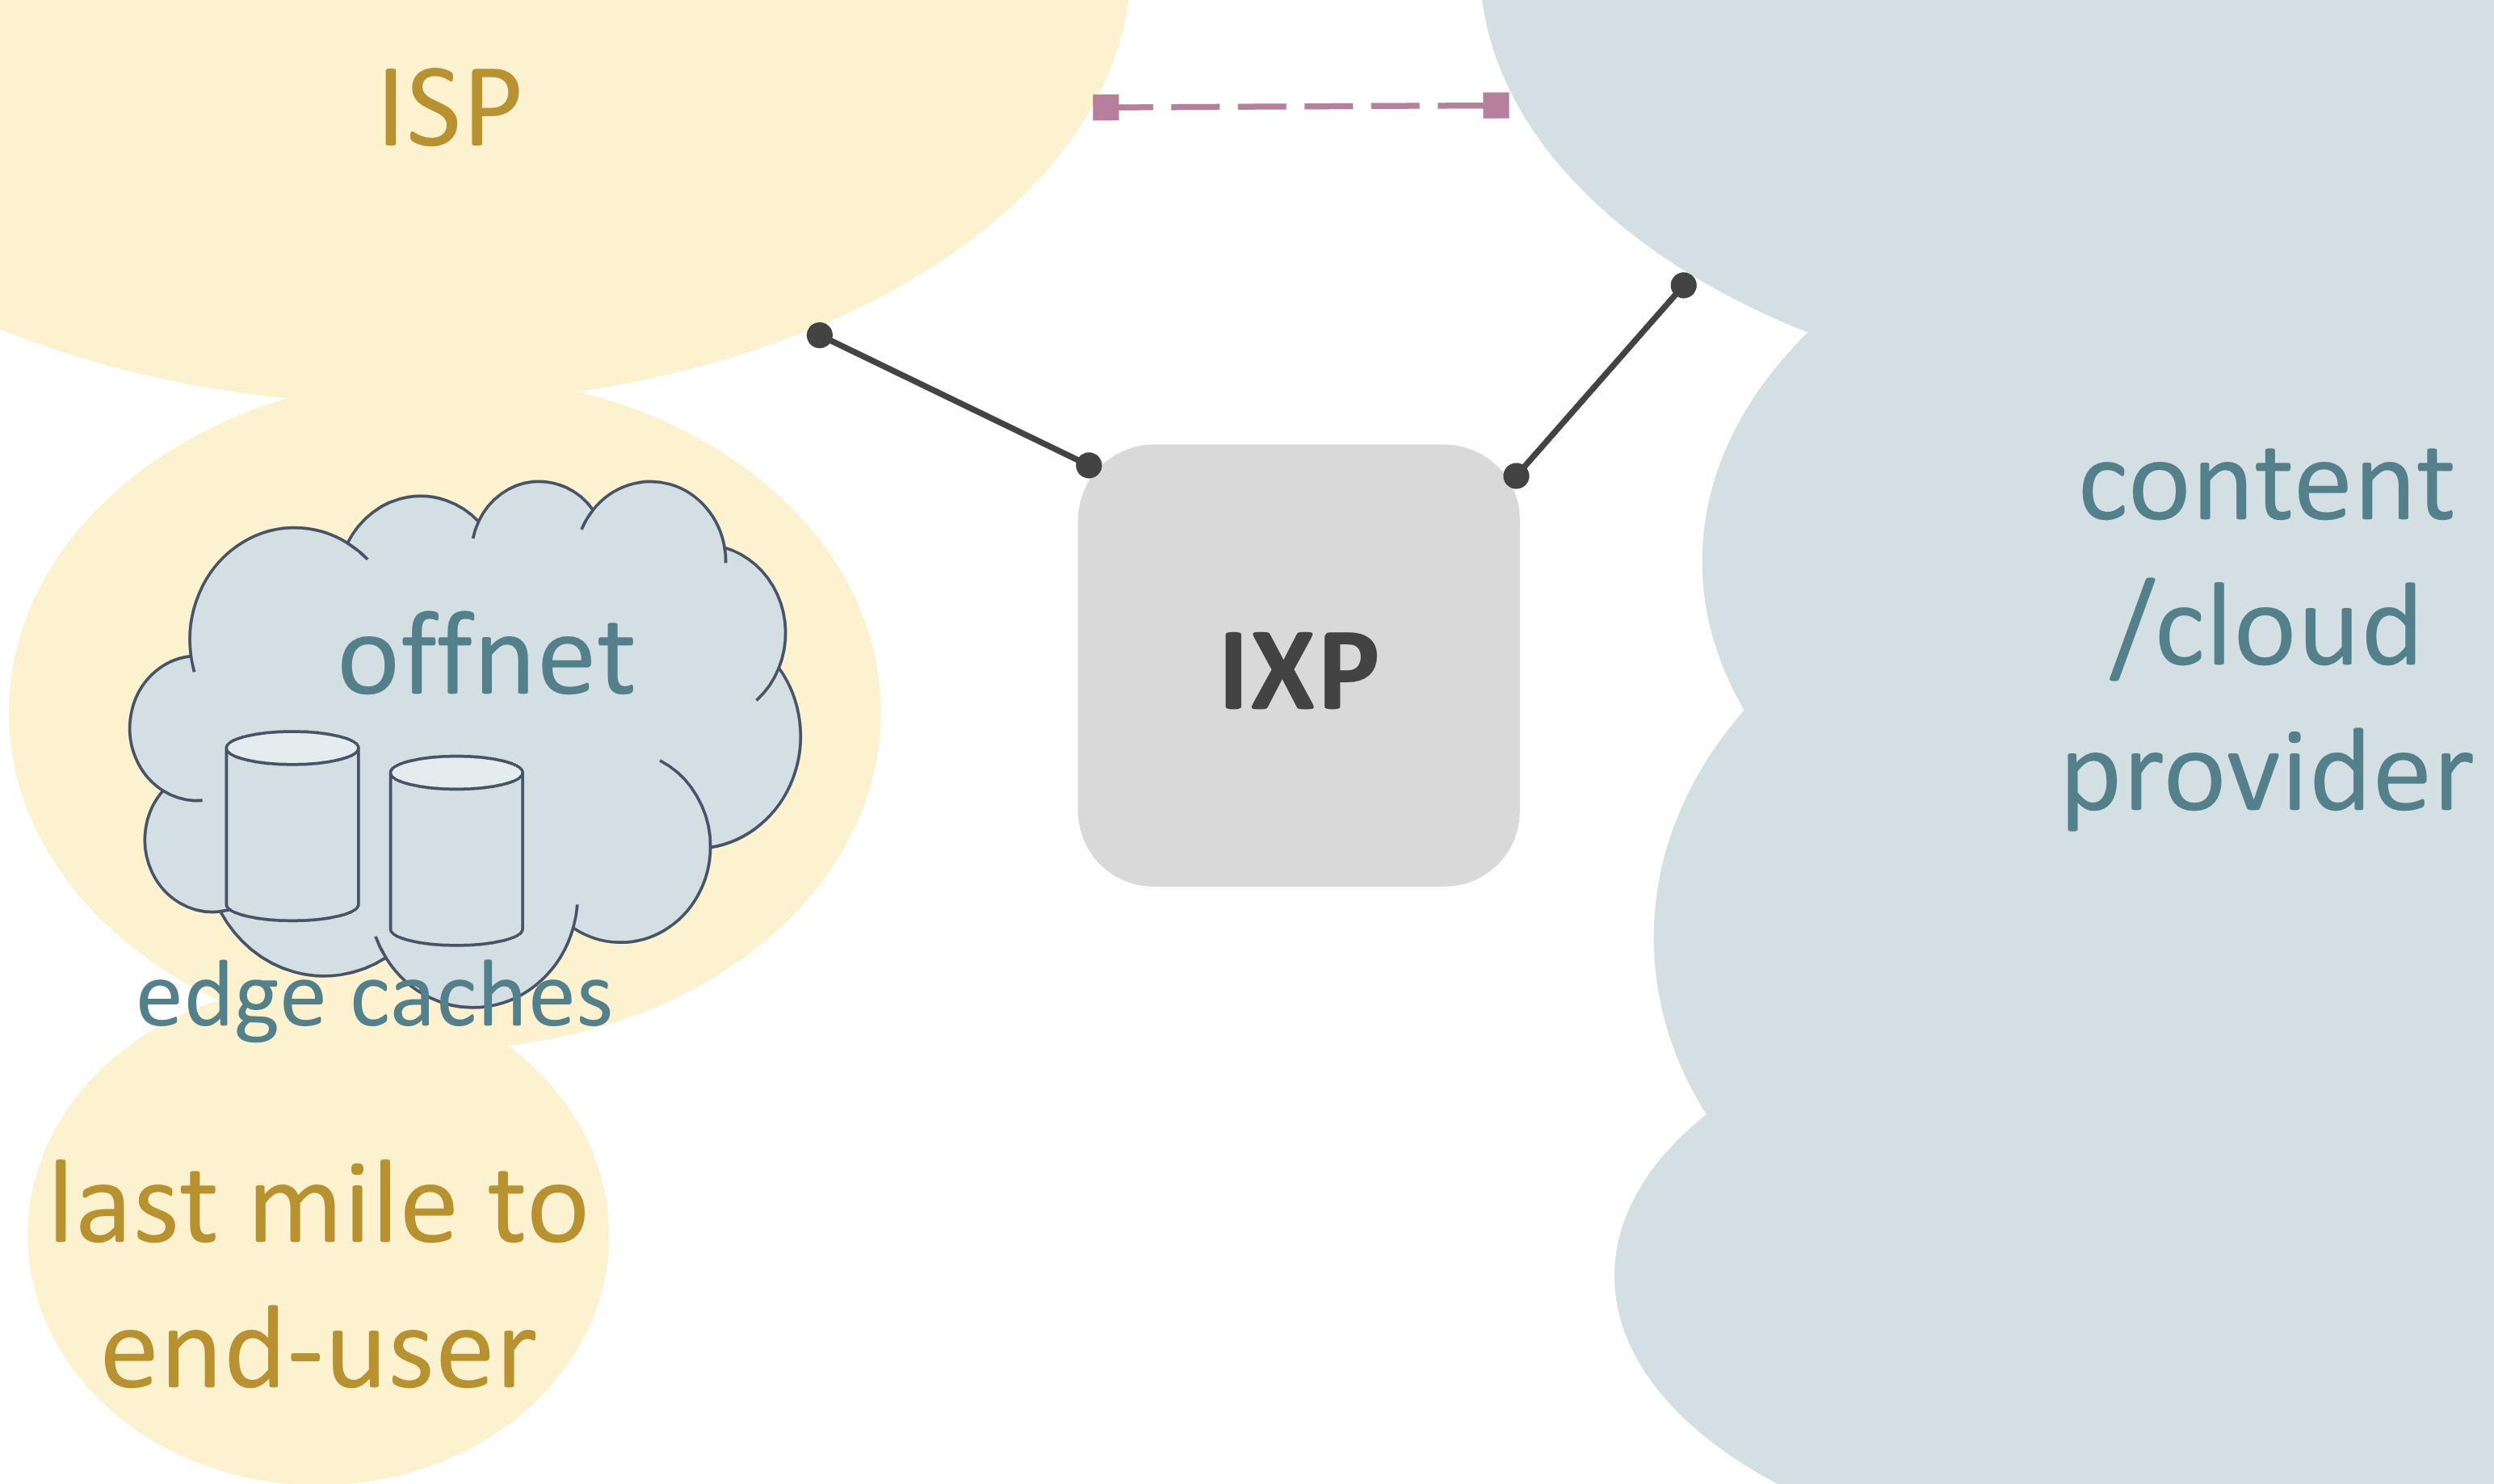
\includegraphics[width=0.60\textwidth]{images/ixp-ccp-edge.png}
  \end{center}

\begin{enumerate}
  \item Directly connect their data-centres to large ISPs and IXPs.
  \item Peer with ISPs to minimise transit cost and latency.
  \item Deploy \textbf{edge caches} \emph{inside} ISP networks to store
        popular content close to users.
  \item Interconnect those caches via an \textbf{off-net}―a private
        overlay that is \emph{logically} theirs but \emph{physically}
        located within partner ISPs.
\end{enumerate}



%---------------------------------------------------------------
\subsection{Edge Caches and Off-nets}\label{subsec:edge}
\begin{definition}
  \textbf{Edge cache}: server cluster owned and managed by the content
  provider but \emph{installed within} the ISP's premises; stores the
  most popular objects for that ISP's subscribers.
\end{definition}
\vspace{10px}

\begin{definition}
  \textbf{Off-net}: the private backbone interconnecting multiple edge
  caches that reside \emph{outside} the content provider's core
  network.
\end{definition}

This arrangement improves user experience while reducing upstream
traffic for the ISP.

%---------------------------------------------------------------
\subsubsection*{Recap}\label{sssec:recap}
\begin{enumerate}
  \item The Internet scales through a three-tier ISP hierarchy
        (access–regional–tier-1) governed by customer–provider
        contracts.
  \item Peering offers a cost-effective shortcut whenever traffic
        volumes justify it.
  \item IXPs simplify physical connectivity by acting as neutral
        switching hubs.
  \item Large content/cloud providers now run quasi-global networks,
        peer with ISPs, and deploy edge caches/off-nets for performance.
\end{enumerate}
\newpage
%--------------------------------------------------------------------
\section{The Network Interface and the CPU}\label{sec:nic-cpu}
Every Internet message created by a user process must travel from
\emph{main memory} to the \emph{Network Interface Card~(NIC)}, descend
through the five protocol layers, and finally leave the machine as a
physical signal.  This section shows how the operating system, the NIC,
and the layered “network stack” cooperate to make that happen.

%--------------------------------------------------------------------
\subsection{Hardware Overview}\label{subsec:nic-hw}

\begin{description}
  \item[NIC controller] On-board processor that handles packet queues and
        offloads work from the CPU.
  \item[I/O controller] CPU’s gateway to peripheral devices.
  \item[DMA controller] Copies data between main memory and device
        memory \emph{without} CPU intervention.
\end{description}
\begin{center}
  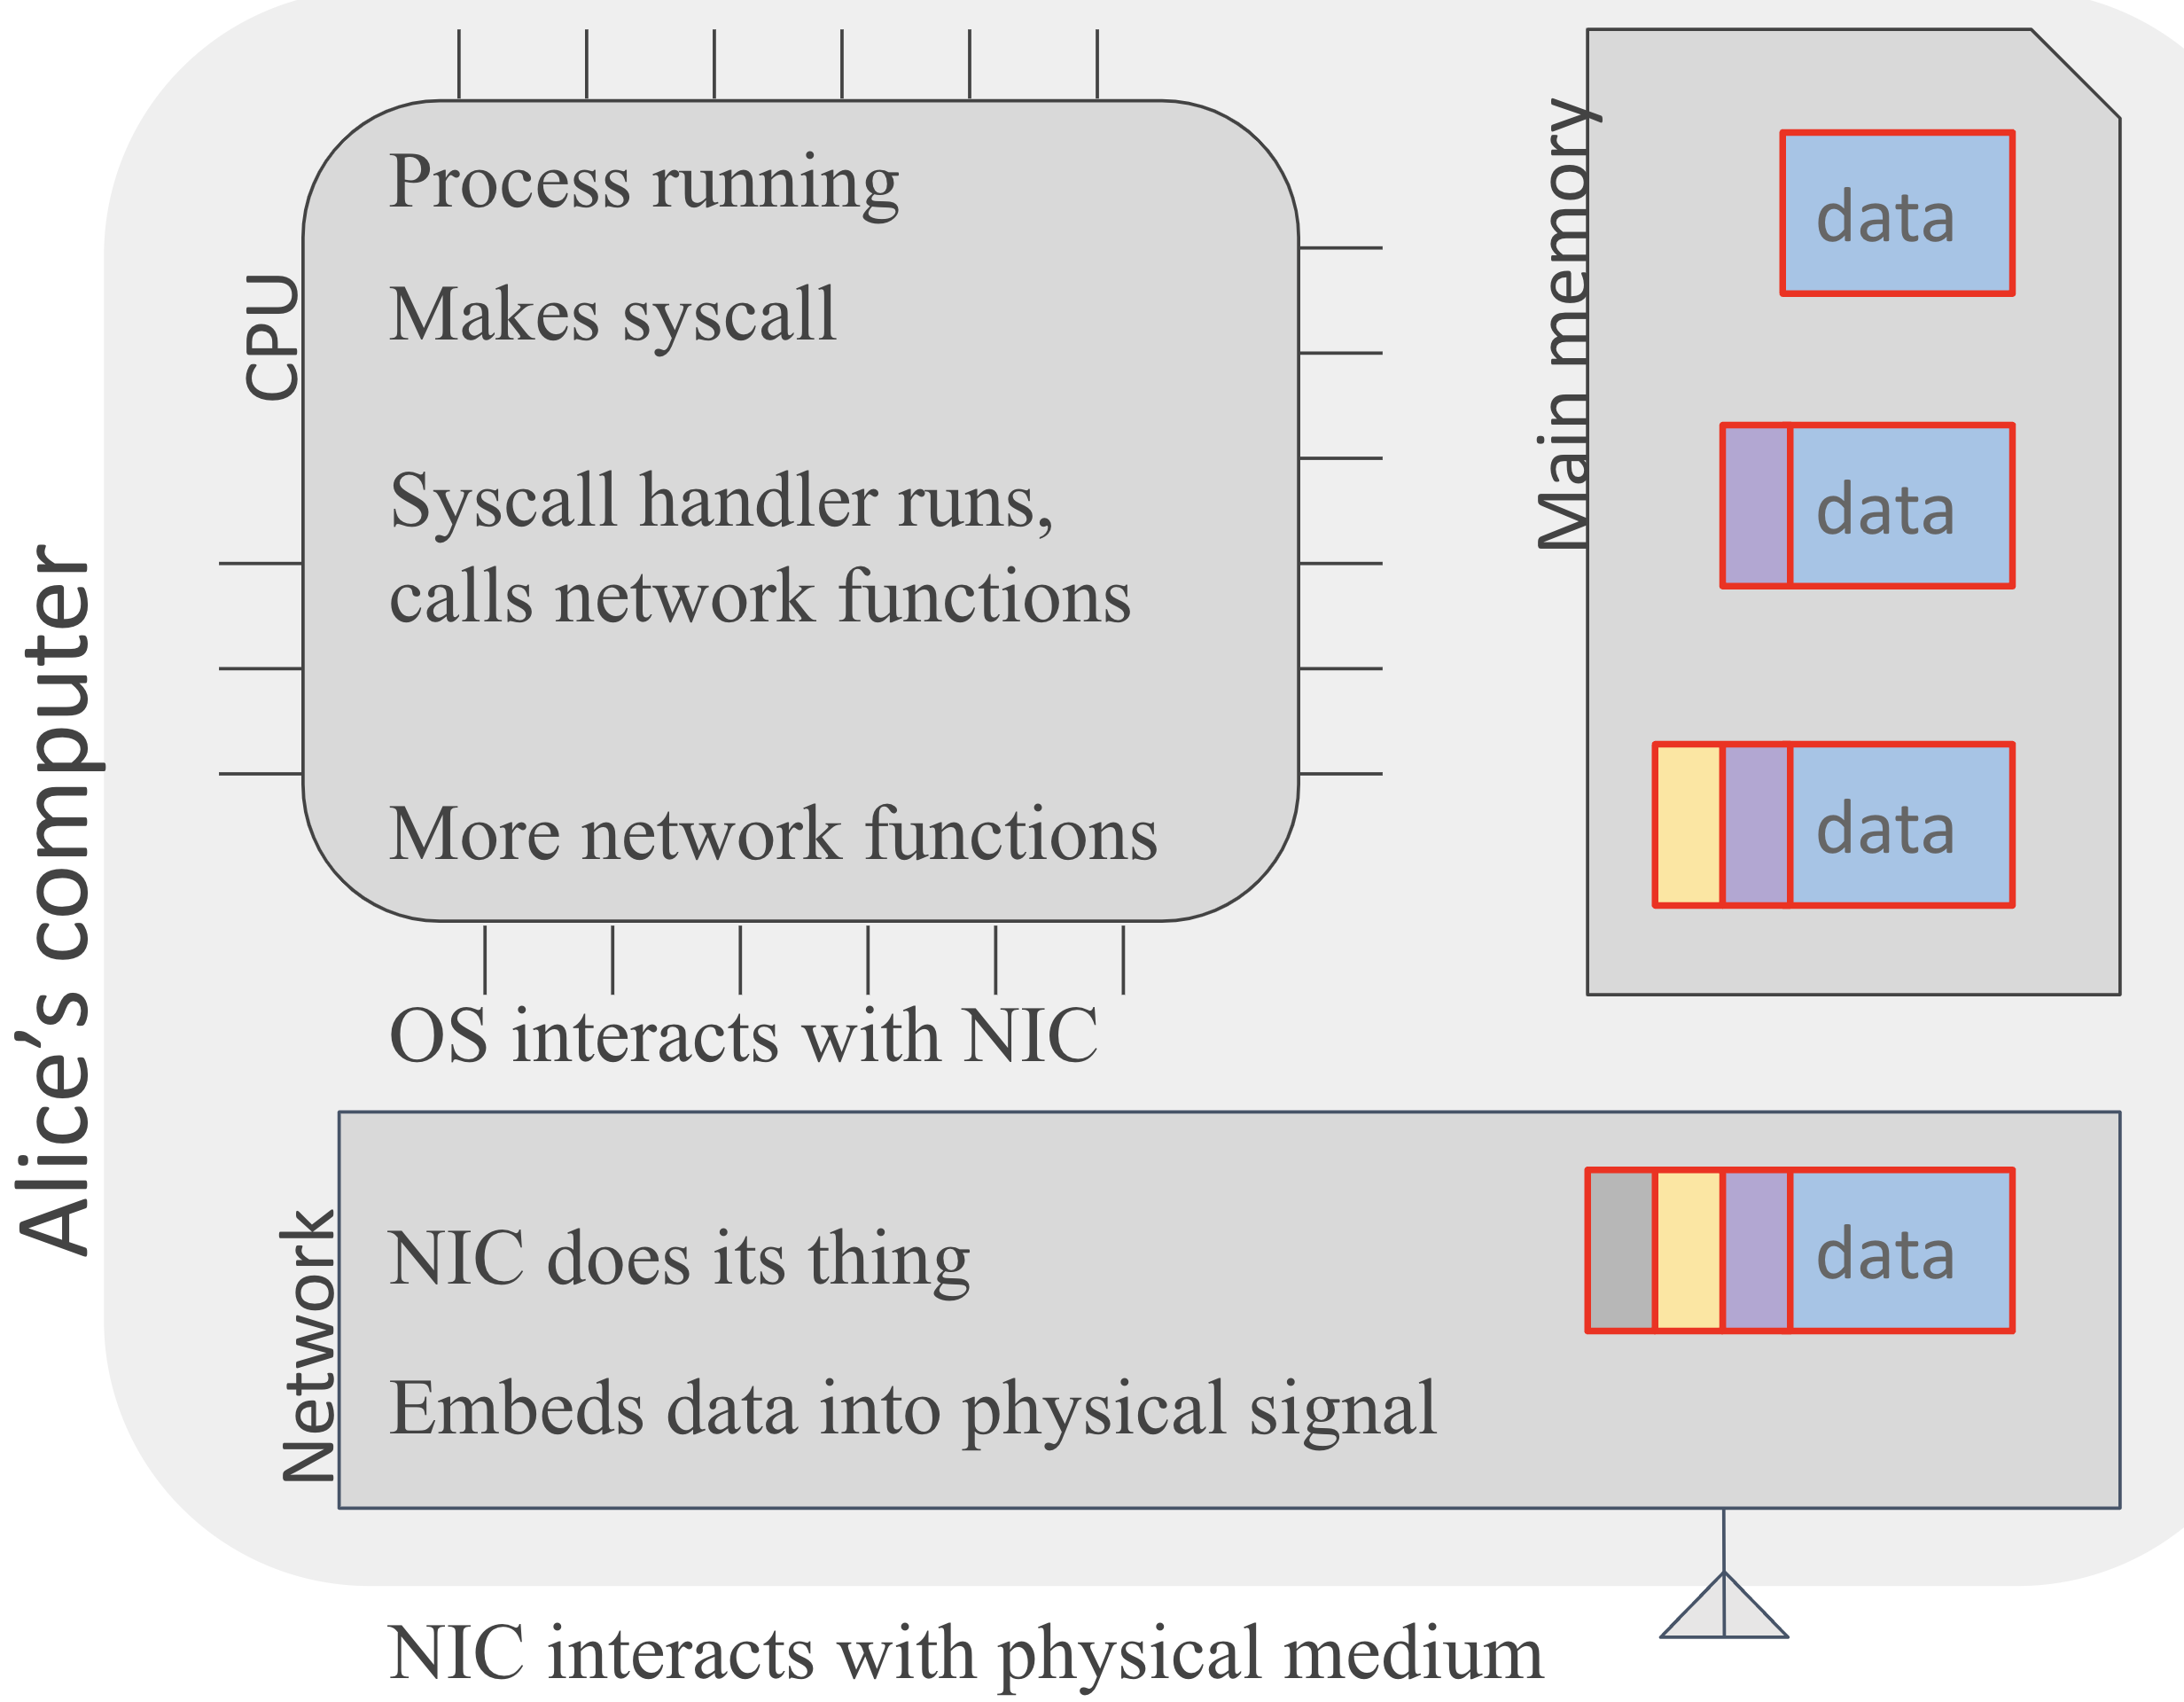
\includegraphics[width=0.60\textwidth]{images/nic.png}
\end{center}

\noindent
\textbf{Send path (user process $\rightarrow$ wire):}
\begin{enumerate}
  \item User process issues a \texttt{sendto()} \emph{network
        syscall}; CPU traps into \emph{kernel mode}.
  \item Kernel prepends \emph{transport} and \emph{network} metadata to
        the user data.
  \item Kernel programs the I/O controller; DMA copies the buffer to NIC
        memory.
  \item NIC adds a \emph{link-layer} header, forming a
        \textbf{packet} = \emph{payload $+$ all headers}.
  \item NIC converts the packet bits into an electrical/optical/radio
        signal and transmits it onto the medium.
\end{enumerate}
\newpage
%--------------------------------------------------------------------
\subsection{The Five-Layer Internet Stack}

\begin{description}
  \item[Application] User programs (web, chat, file-transfer).
  \item[Transport] TCP and UDP.
  \item[Network] IP (Internet Protocol).
  \item[Link] Ethernet, Wi-Fi, DOCSIS, DSL, \dots
  \item[Physical] Copper wire, fibre optics, radio, free-space optics.
\end{description}
\begin{minipage}[htp]{0.45\textwidth}
\begin{center}
  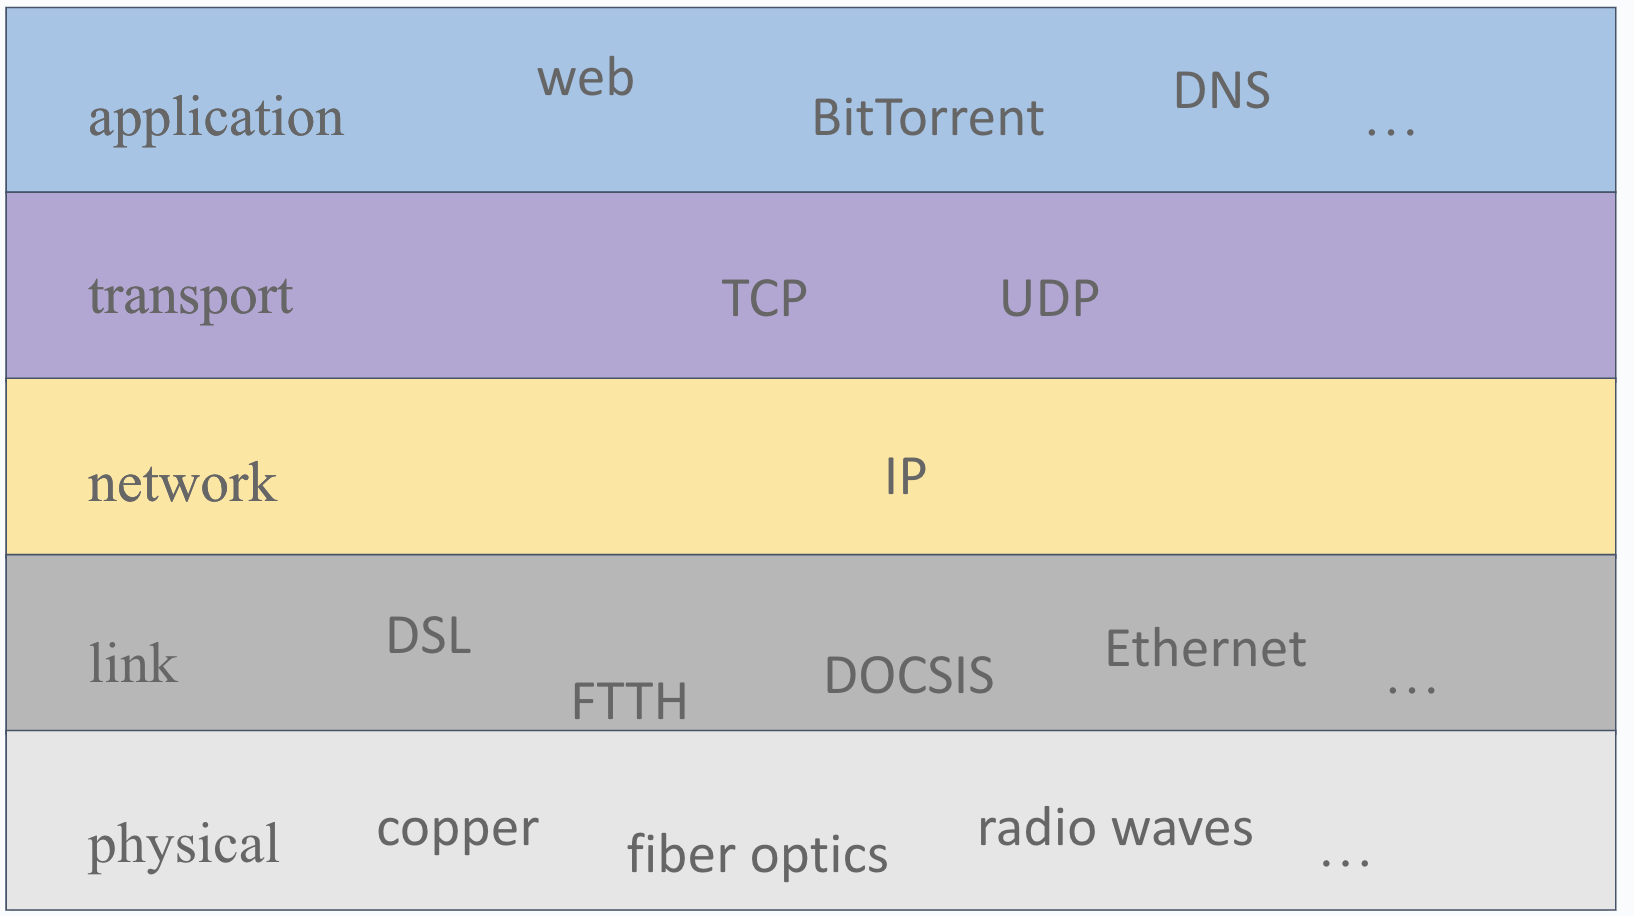
\includegraphics[width=1\textwidth]{images/nic-tech.png}
\end{center}
\end{minipage}
\begin{minipage}[htp]{0.45\textwidth}
\textbf{Layer Properties}
\begin{itemize}
  \item[-] \textbf{Abstraction}: each layer hides lower-level details from
        the layer above.
  \item[-] \textbf{Encapsulation}: a layer \emph{prepends} its own header.
  \item[-] \textbf{Decapsulation}: a layer \emph{removes} its header on the
        receiving host.
  \item[-] \textbf{Interfaces}: adjacent layers communicate through a
        well-defined API (e.g.\ a \emph{syscall} between Application and
        Transport).
\end{itemize}
\emph{Layers reduce complexity and increase flexibility; they do not
directly improve raw performance.}
\end{minipage}
%--------------------------------------------------------------------
\begin{example}[EPFL Web Server]
  \noindent
  Consider the machine that answers HTTP requests for
  \texttt{www.epfl.ch}.  Important naming facts:\\

  \begin{minipage}[htp]{0.45\textwidth}
    \begin{center}
      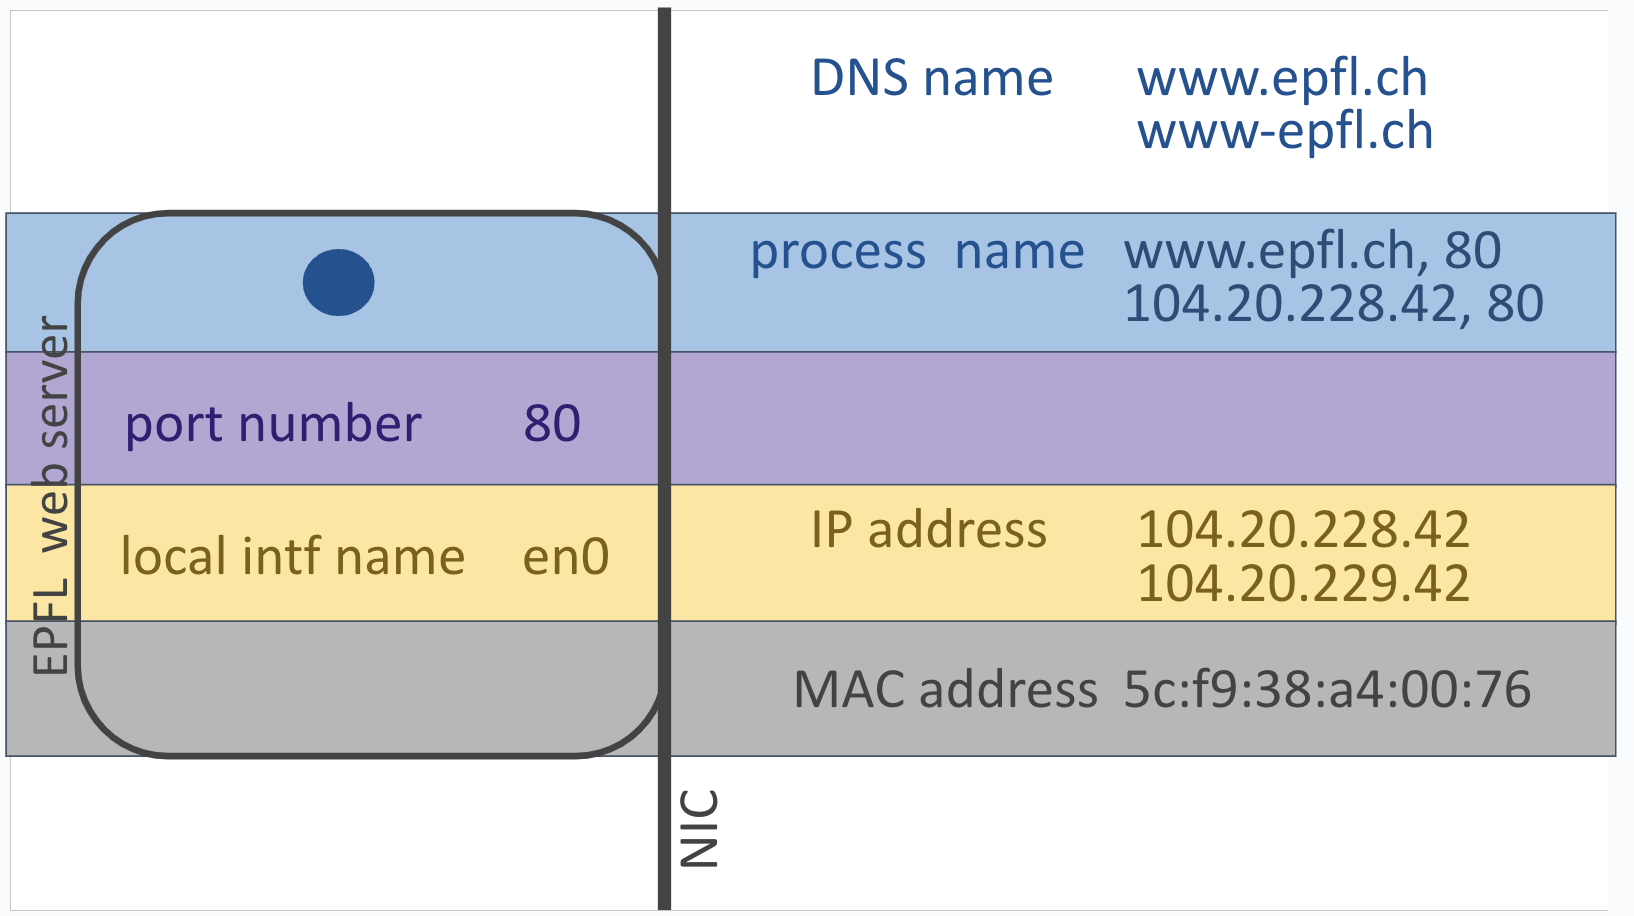
\includegraphics[width=1.2\textwidth]{images/epfl-example.png}
    \end{center}
    \end{minipage}
    \hfill
  \begin{minipage}[htp]{0.45\textwidth}
    \small
  \begin{enumerate}

    \item \textbf{Application layer}  - Runs a web–server \emph{process}.
            
    \item \textbf{Transport layer}  
          \begin{itemize}
            \item Identifies that process with \textbf{port
                  \texttt{80}}.  
            \item Other processes on the same host listen on
                  \emph{different} port numbers.
          \end{itemize}
  
    \item \textbf{Network layer}  
          \begin{itemize}
            \item Sees the host’s network interface as \texttt{en0}.
            \item Associates one or more \textbf{IP addresses} with
                  \texttt{en0} (e.g.\ \texttt{104.20.228.42}).
          \end{itemize}
  
    \item \textbf{Link layer}  
          \begin{itemize}
            \item Uses a globally–unique \textbf{MAC address}
                  (e.g.\ \texttt{5c:f9:38:a4:00:76}) for the same
                  interface.
          \end{itemize}
  \end{enumerate}
  \end{minipage}\\
  \end{example}
  %--------------------------------------------------------------------
  \subsubsection{Name Identifiers}\label{subsec:names}
  \begin{itemize}
    \item[-] \textbf{Interface identifiers}  
          \begin{description}
            \item[DNS name] Human-readable alias
                  (\texttt{www.epfl.ch}).
            \item[IP address] Network-layer locator
                  (\texttt{104.20.228.42}).
            \item[MAC address] Link-layer locator
                  (\texttt{5c:f9:38:a4:00:76}).
            \item[OS handle] Local label (e.g.\ \texttt{en0}).
          \end{description}
    \item[-] \textbf{Process identifier} $
            \textit{interface–name} \; , \; \textit{port}
          $\\
          A two-tuple: first choose the interface by DNS/IP, then the
          process by its port number.
  \end{itemize}
  

  

\end{document}